
\documentclass[a4paper,12pt]{article}
\usepackage{geometry}
\usepackage{enumitem}
\usepackage{fancyhdr}
\usepackage{xcolor}
\usepackage{sectsty}
\usepackage{multicol}
\usepackage{graphicx}
\usepackage{amsmath}
\usepackage{float}
\usepackage{tikz}
\usetikzlibrary{shapes,arrows}
\def\inputGnumericTable{}
\usepackage[latin1]{inputenc}
\usepackage{fullpage}
\usepackage{color}
\usepackage{array}
\usepackage{longtable}
\usepackage{calc}
\usepackage{multirow}
\usepackage{hhline}
\usepackage{ifthen}
\geometry{top=1in, bottom=1.5cm, left=1.5cm, right=1.5cm}
\pagestyle{empty}
\sectionfont{\color{blue}}

\begin{document}

\thispagestyle{fancy}
\fancyhf{}
\fancyhead[L]{\textbf{IIITB - COMET}}
\fancyhead[L]{
\includegraphics[width=4cm, height = 1cm]{logo.png}}
\fancyhead[R]{Name: HEMANTH.T \\ Batch: COMETFWC033 \\ Date: 04 September 2025}
\renewcommand{\headrulewidth}{0pt}
\fancyfoot[C]{\thepage}
\vspace*{1cm}

\begin{center}
    {\LARGE \textbf{\textcolor{blue}{GATE 2018 ph, Question 13 --- Detailed Analysis}}}
\end{center}

\section*{\textbf{Question 13}}
A 2-to-1 multiplexer selects between inputs \(A_0\) and \(A_1\) using select line \(C\). The output is \(X = A_0\) when \(C=0\) and \(X = A_1\) when \(C=1\). Which gate-level implementation corresponds to this behavior?

\section*{\textbf{Short Answer}}
The canonical implementation is:
\[
\boxed{\,X \;=\; \overline{C}\,A_0 \;+\; C\,A_1\,}
\]
(That is, invert \(C\); AND \(\overline{C}\) with \(A_0\); AND \(C\) with \(A_1\); OR the results.)

\section*{\textbf{Detailed Analysis and Derivation}}

\textbf{1. Reasoning from the specification:}

- Required behavior:
  \begin{itemize}
    \item If \(C = 0\) then \(X = A_0\).
    \item If \(C = 1\) then \(X = A_1\).
  \end{itemize}

- A standard way to encode a select is:
  \[
  X = (\text{select for }A_0)\cdot A_0 \;+\; (\text{select for }A_1)\cdot A_1.
  \]
  Here the select for \(A_0\) is \(\overline{C}\) and for \(A_1\) is \(C\). Hence:
  \[
  X = \overline{C}A_0 + C A_1.
  \]

\textbf{2. Check by cases:}
\[
\begin{aligned}
C=0 &\implies X = \overline{0}A_0 + 0\cdot A_1 = 1\cdot A_0 + 0 = A_0,\\
C=1 &\implies X = \overline{1}A_0 + 1\cdot A_1 = 0\cdot A_0 + A_1 = A_1.
\end{aligned}
\]
Hence the expression is correct.

\section*{\textbf{Truth Table}}

Here is the full truth table listing all combinations of \(A_0, A_1, C\) and resulting \(X\):

\begin{center}
\begin{tabular}{|c|c|c|c|}
\hline
$A_0$ & $A_1$ & $C$ & $X$ \\ \hline
0 & 0 & 0 & 0 \\ \hline
0 & 0 & 1 & 0 \\ \hline
0 & 1 & 0 & 0 \\ \hline
0 & 1 & 1 & 1 \\ \hline
1 & 0 & 0 & 1 \\ \hline
1 & 0 & 1 & 0 \\ \hline
1 & 1 & 0 & 1 \\ \hline
1 & 1 & 1 & 1 \\ \hline
\end{tabular}
\end{center}

\textbf{Explanation of rows:}
- Rows where \(C=0\): \(X = A_0\) (rows 1,3,5,7).
- Rows where \(C=1\): \(X = A_1\) (rows 2,4,6,8).

\section*{\textbf{Sum-of-Minterms Form (optional)}}
If you want minterms (3 variables \(A_0,A_1,C\) ordered as \([A_0\,A_1\,C]\)), \(X=1\) for combinations:
- \([0\,1\,1]\) decimal \(3\),
- \([1\,0\,0]\) decimal \(4\),
- \([1\,1\,0]\) decimal \(6\),
- \([1\,1\,1]\) decimal \(7\).

So one can write:
\[
X = \sum m(3,4,6,7),
\]
which simplifies back to \(X=\overline{C}A_0 + C A_1\).

\section*{\textbf{Gate-Level Implementation (diagram)}}
Below is a simple gate-level schematic drawn using basic TikZ shapes (no special gate library required).  
(Notation: rectangles labeled AND/OR/NOT are used to represent gates.)

\begin{center}
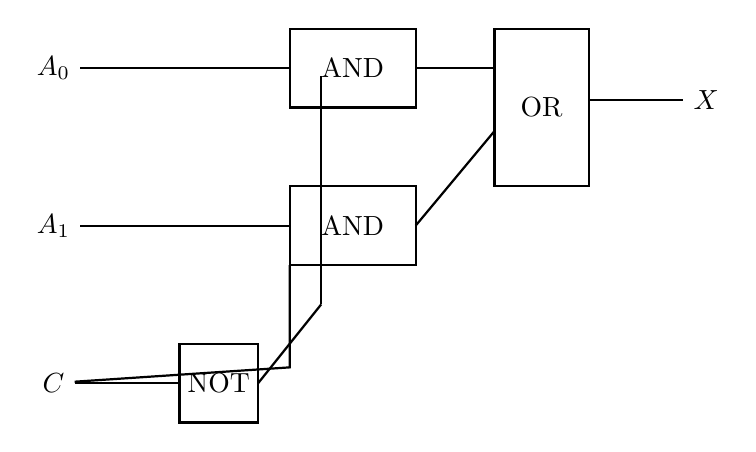
\begin{tikzpicture}[thick, scale=1, every node/.style={transform shape}]
    % Inputs
    \node (A0) at (0,2) {$A_0$};
    \node (A1) at (0,0) {$A_1$};
    \node (C)  at (0,-2) {$C$};

    % NOT gate (rectangle labeled NOT)
    \draw (1.6,-2.5) rectangle (2.6,-1.5) node[midway]{NOT};
    \draw (C) -- (1.6,-2);

    % wire from NOT to AND0
    \draw (2.6,-2) -- (3.4,-1.0);

    % AND gate for A0 path (rectangle labeled AND)
    \draw (3,1.5) rectangle (4.6,2.5) node[midway]{AND};
    \draw (A0) -- (3,2);
    \draw (3.4,-1.0) -- (3.4,1.9); % connects inverted C to AND A0
% AND gate for A1 path
    \draw (3,-0.5) rectangle (4.6,0.5) node[midway]{AND};
    \draw (A1) -- (3,0);
    \draw (C) -- (3.0,-1.8) -- (3.0,-0.5) ; % connect C to AND for A1

    % OR gate (rectangle labeled OR)
    \draw (5.6,0.5) rectangle (6.8,2.5) node[midway]{OR};
    \draw (4.6,2.0) -- (5.6,2.0); % from AND A0
    \draw (4.6,0.0) -- (5.6,1.2); % from AND A1 (slanted)

    % Output
    \draw (6.8,1.6) -- (8,1.6) node[right]{$X$};
\end{tikzpicture}
\end{center}

\section*{\textbf{Implementation Steps (practical)}}
If you were to implement this on breadboard or in a simple digital trainer:
\begin{enumerate}
    \item Use one inverter (NOT) for the select line \(C\) to obtain \(\overline{C}\).
    \item Use two 2-input AND gates:
    \begin{itemize}
        \item AND1: inputs \(\overline{C}\) and \(A_0\) $\rightarrow$ output \(T_0\).
        \item AND2: inputs \(C\) and \(A_1\) $\rightarrow$ output \(T_1\).
    \end{itemize}
    \item Use one 2-input OR gate: OR inputs \(T_0, T_1 \rightarrow X\).
\end{enumerate}
\begin{center}
  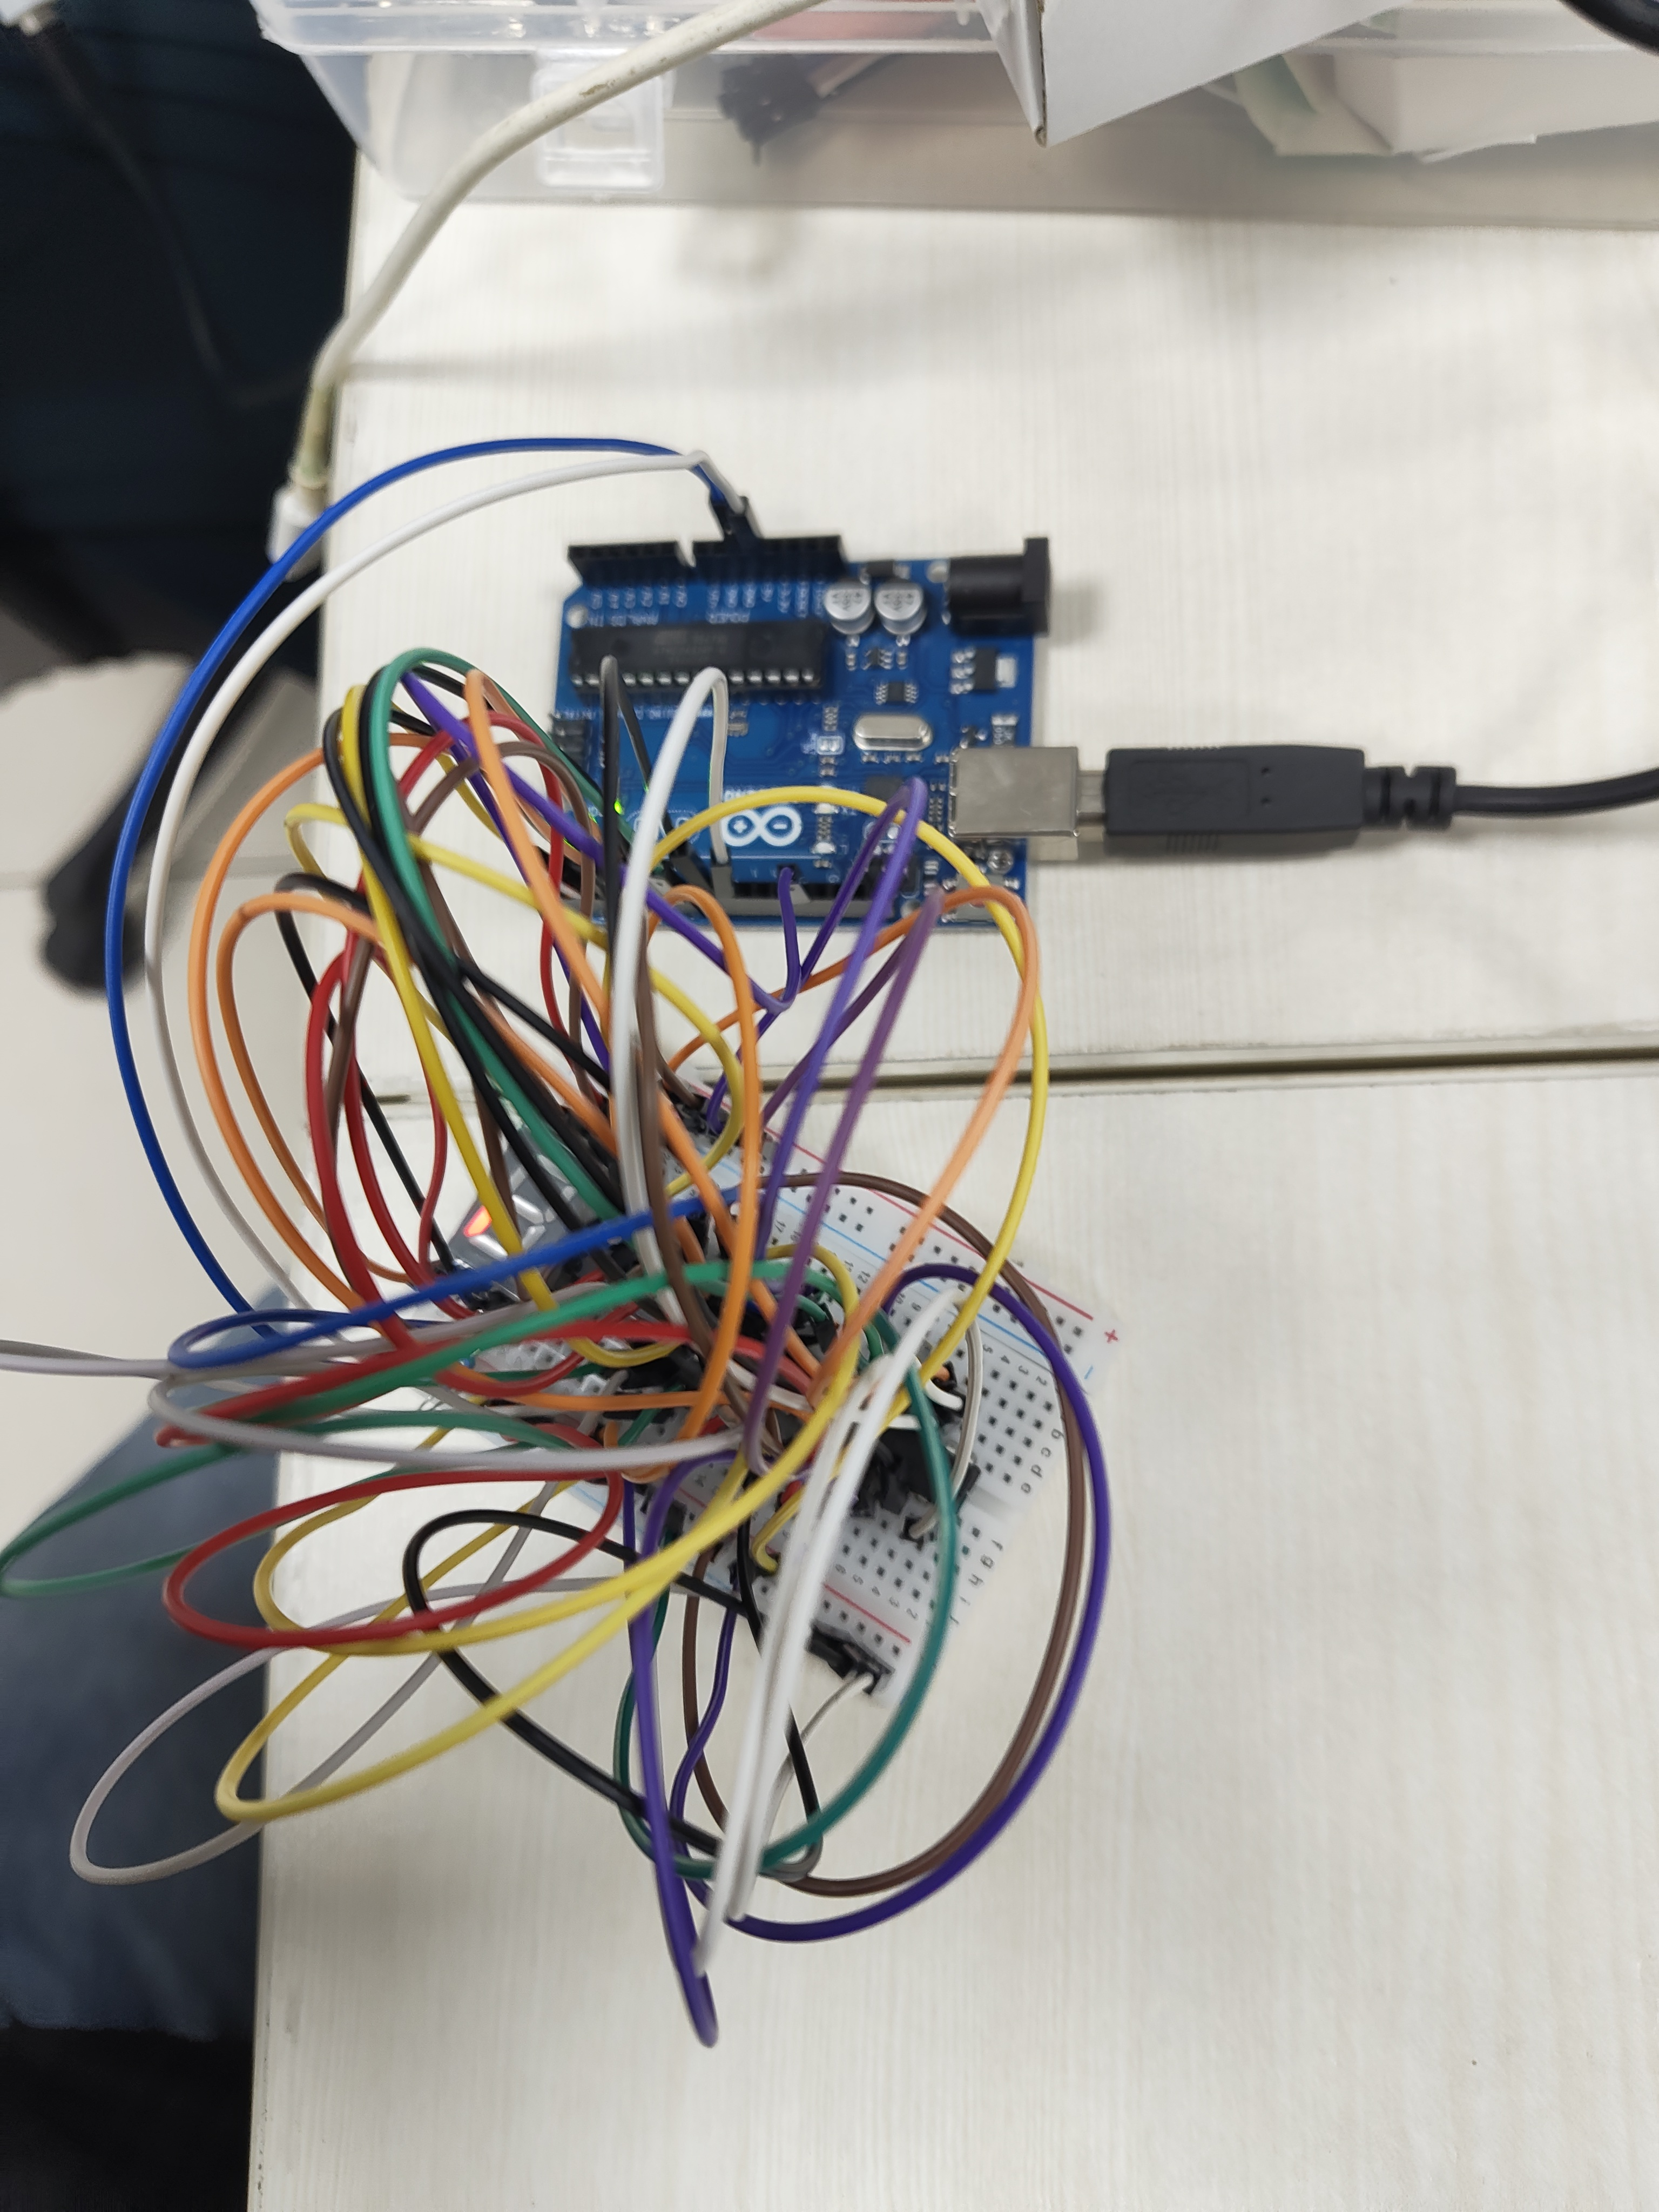
\includegraphics[width=12cm, height=12cm]{output.jpg}
\end{center}
\section*{\textbf{Conclusion}}
\begin{itemize}
    \item The multiplexer equation \(X=\overline{C}A_0 + C A_1\) correctly implements the required selection behavior.
    \item The full truth table above confirms the mapping of inputs to output for all input combinations.
    \item The gate-level implementation uses one inverter, two ANDs and one OR (standard, minimal realization).
\end{itemize}

\end{document}
